\documentclass[12pt,a4paper]{article} %(nie wiem kiedy) usunąłem tą linię i nie wiem czy tak było
%przykladowe pakiety
\usepackage[utf8]{inputenc}
\usepackage{polski}
\usepackage{graphicx}
\usepackage{caption}
\usepackage{amsmath} % w zasadzie tez mozna wywalic 
\usepackage{booktabs}
\usepackage{listings}
\usepackage{color}
\usepackage{geometry} 
\usepackage{biblatex}
\addbibresource{references.bib}
\usepackage{hyperref}
\usepackage{subcaption}

\lstset{language=C++,backgroundcolor=\color[rgb]{0.99,0.99,0.99},captionpos=b,tabsize=3,numbers=left,numberstyle=\tiny,numbersep=5pt,basicstyle=\footnotesize,keywordstyle=\color[rgb]{0,0,1},commentstyle=\color{Darkgreen},stringstyle=\color{red},numbers=left,xleftmargin=2em,framexleftmargin=1.8em,}
 \newgeometry{tmargin=3cm, bmargin=3cm, lmargin=2cm, rmargin=2cm} 
\definecolor{zielony}{rgb}{0,1,0}

\geometry{
	a4paper,
	left = 2.5cm,
	right = 2.5cm,
	top = 2cm,
	bottom = 2cm
}

\begin{document}

\begin{titlepage}

\newcommand{\HRule}{\rule{\linewidth}{0.5mm}}

\center
 
\textsc{\LARGE Politechnika Wrocławska}\\[1.5cm] 
\textsc{\Large Zastosowanie informatyki w gospodarce}\\[0.5cm]

\HRule \\[0.5cm]
{ \huge \bfseries Relacje pomiędzy bytami w tekstach literackich - dokumentacja}\\[0.2cm]
\HRule \\[1.6cm]
 
 
\begin{minipage}{0.4\textwidth}
\begin{flushleft} \large
\emph{Lider grupy:}\\
Przemysław \textsc{Wujek} 234983\\
\emph{Skład grupy:}\\
Paweł \textsc{Czarnecki} 234974\\
Łukasz \textsc{Łupicki} 257536\\
Dawid \textsc{Piechota} 235851\\
Bartosz \textsc{Rodziewicz} 226105\\
Wojciech \textsc{Wójcik} 235621\\
\end{flushleft}
\end{minipage}
~
\begin{minipage}{0.4\textwidth}
\begin{flushright} \large
\emph{Prowadzący:} \\
dr inż. Tomasz \textsc{Walkowiak} 
\end{flushright}
\end{minipage}\\[4cm]

\vfill
{\large 15 kwietnia 2020}

\end{titlepage}
   
\newpage
\tableofcontents 

\newpage

\section{Zadanie programu}
    Zadaniem stworzonej aplikacji jest analiza tekstów literackich, która polega na wykryciu bytów, wyznaczeniu ich częstości występowania oraz powiązań pomiędzy nimi. Aplikacja wykorzystuje narzędzie \textit{NER} udostępniane przez \textit{clarin-pl}.\\
    Aplikacja klienta umożliwia wgranie tekstu, którego wyniki analizy zostają zaprezentowane w postaci grafu. Zaimplementowane funkcje umożliwiają przeglądanie oraz edycję prezentowanego grafu.\\
    Użytkownik posiada możliwość zapisu do pliku edytowanego grafu. Dodatkowo aplikacja przechowuje w bazie danych wcześniej przeanalizowane grafy, aby użytkownik nie musiał zlecać zadania analizy tego samego tekstu dwa razy.

\section{Link do repozytorium projektu}
    \url{https://github.com/Isild/ZIWG}

\section{Technologia}
    Część serwerowa aplikacji zaimplementowana została z wykorzystaniem języka Python wraz z frameworkiem Flask.\\
    Część kliencka wykorzystuje bibliotekę Vue.

\section{Uruchomienie}

    \subsection{Uruchamianie ręczne}
    %tutaj nawet komendy wystarczą bez długiego opisu
    % BAATO: moge to zrobic (w sensie odpalanie na linuxie/windowsie), ale dopiero po 22 jakos. swoja czesc wczytywania pliku wraz z przekierowaniem chyba wystarczajaco opisalem
        Po pobraniu projektu z repozytorium z githuba należy uruchomić aplikację serwera oraz aplikację klienta.\\
        Aplikacja klienta znajduje się w katalogu \textit{/client}. W owym katalogu także znajduje się \textit{README.md} w którym umieszczono instukcję uruchomienia aplikacji.\\
        
        \begin{lstlisting}[caption={Komendy budujące aplikacje klienta}, label={zad1}, captionpos=t]
# Komenda instalujaca wszystkie potrzebne biblioteki

yarn install

# Komenda kompilujaca aplikacje w trybie developmentu

yarn serve

# Komenda budujaca aplikacje w trybie produkcyjnym

yarn build
        \end{lstlisting}
        Aplikacja serweru znajduje się w katalogu \textit{/server}. Tutaj także umieszczony jest plik \textit{ReadMe.md} zawierający instrukcję instalacji oraz uruchomienia aplikacji.\\
\newpage
        \begin{lstlisting}[caption={Komendy budujące aplikacje serwera}, label={zad1}, captionpos=t]
0.  Upewnij sie ze posiadasz zainstalowanego python3, pip i virtualenv
1.  Tworzenie venv  
    **_Linux_**  
    
    $ python3 -m venv env
    $ source env/bin/activate
    
    **_Windows_**  
    
    $ py -m venv env
    $ .\env\Scripts\activate
    
2.  Instalacja wymaganych bibliotek z pliku `requirements.txt`  
    
    (env) $ pip install -r requirements.txt
    
3.  Uruchamianie  
    
    (env) $ python app_run.py run
    
    Podobny komunikat powinien zostac wyswietlony w terminalu jesli aplikacja 
    poprawnie sie uruchomila i dziala:
    
    * Serving Flask app "app.services.app" (lazy loading)
    (...)
    * Running on http://127.0.0.1:5000/ (Press CTRL+C to quit)


# Komenda aplikacji
    run - uruchamia aplikacje serwera, pełne wywolanie 'python app_run.py run'

        \end{lstlisting}
    \subsection{Docker}
    Aplikacja będzie możliwa do uruchomienia za pomocą narzędzia Docker wywołując komendę \textit{docker-compose up}. Nie jest wspierana wersja Docker Toolbox.
\section{Aplikacja}

    \subsection{Menu}
    
    Do poruszania się po aplikacji wykorzystywane jest zwijane menu znajdujące się z prawej strony. Dzięki niemu można przemieszczać się pomiędzy stronami.
            
            \begin{figure}[h!]
                \centering
                \fbox{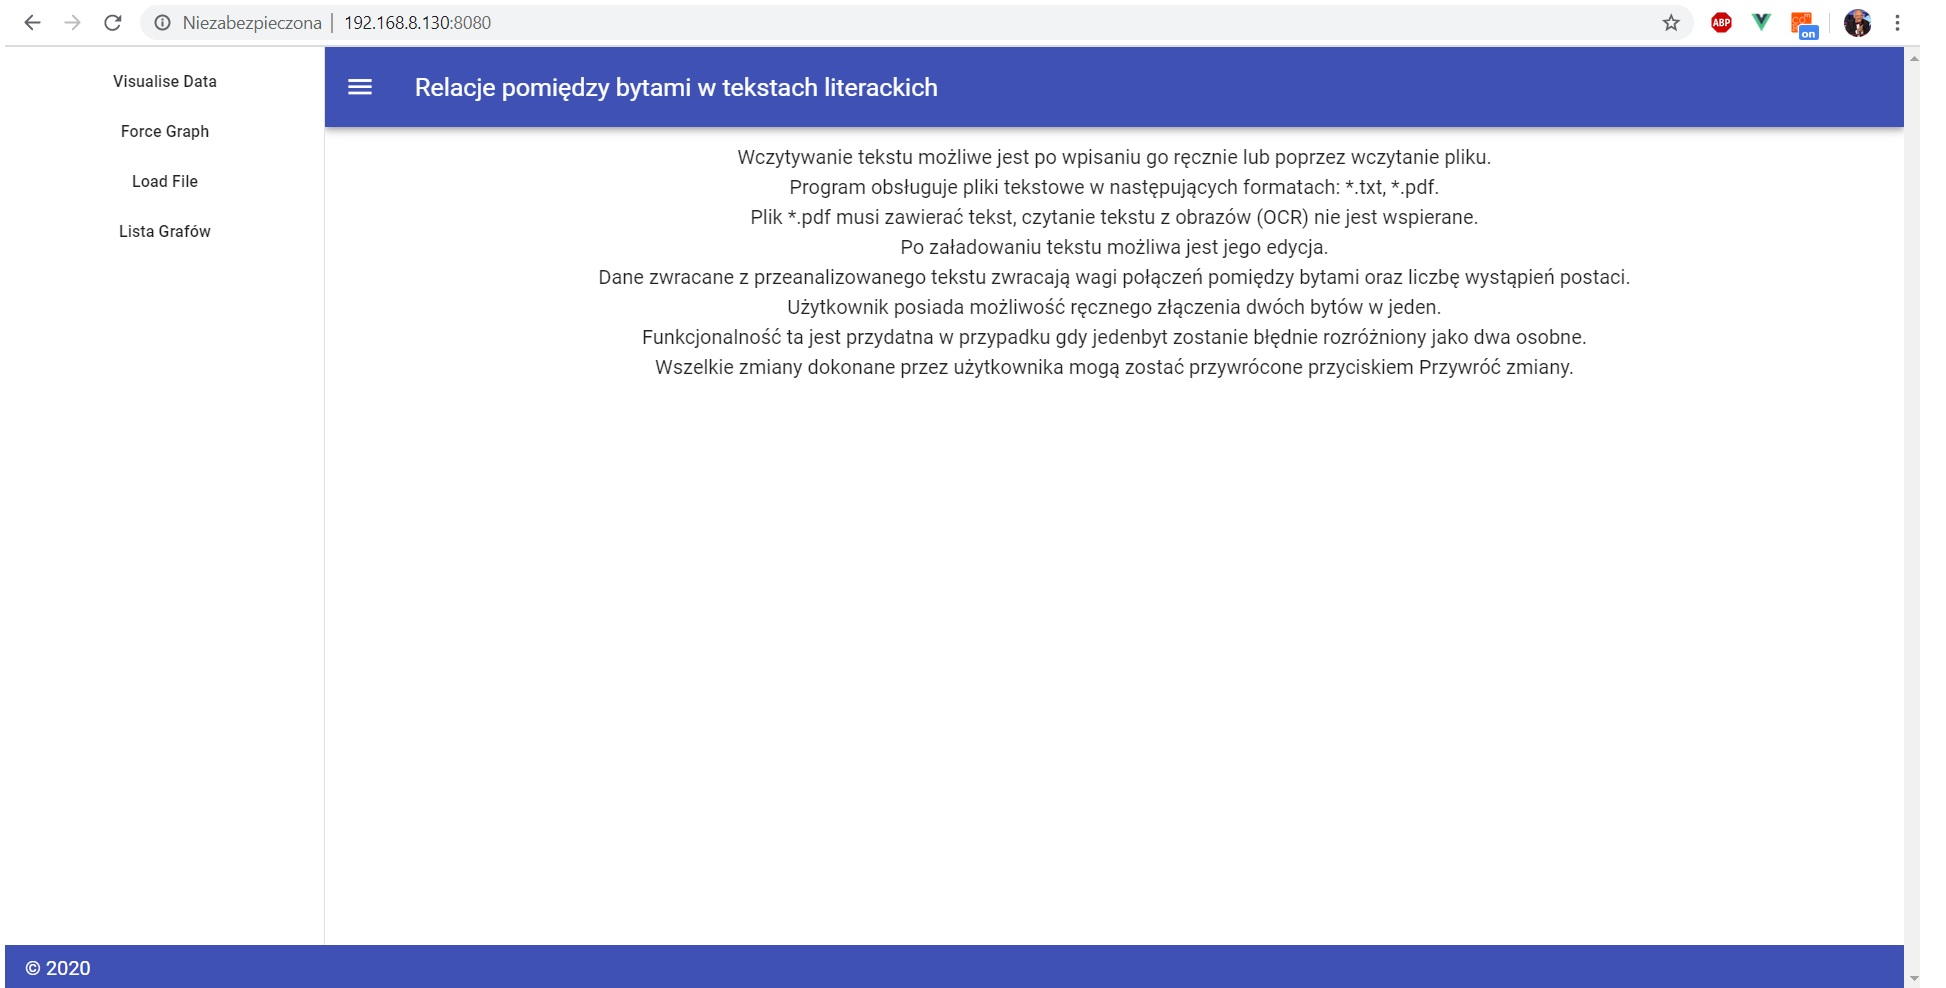
\includegraphics[width=0.9\textwidth]{rys/home.jpg}}
                \caption{Strona domowa aplikacji}
            \end{figure}
            
            
            
    Na stronie domowej znajduje się instrukcja korzystania z programu. Przy użyciu przycisków nawigacji można przechodzić do kolejnych podstron z których można wczytywać tekst lub wyświetlać i edytować grafy.
            
        %opsi zakładek
        
    \subsection{Wczytywanie tekstu do analizy}
        
        Interfejs użytkownika umożliwia wczytywanie tekstu podanego przez użytkownika ręcznie, oraz poprzez wczytanie pliku. Ręczne wczytanie tekstu przez użytkownika polega na wklejeniu tekstu do odpowiedniego miejsca na stronie przeznaczonej do wczytywania. Wczytywanie z pliku polega na wybraniu odpowiedniego pliku, gdzie jego zawartość jest wstawiana w pole na stronie. Umożliwia to jego dalszą edycję, bądź wysłanie.
    
        \subsubsection{Obsługiwane formaty}
            Program aktualnie wspiera wczytywanie tekstu z plików tekstowych (np. txt) oraz plików PDF. Ekstrakcja tekstu z pdf jest wykonywana przez bibliotekę \texttt{pdf.js}. Operacja ta jest wykonywalna lokalnie na komputerze użytkownika. Plik pdf musi zawierać tekst, czytanie tekstu z obrazów (OCR) nie jest wspierane.
        
        \subsubsection{Ręczna modyfikacja}
            Po wczytaniu tekstu jest on uzupełniany do pola, w którym użytkownik może zmienić jego treść, usunąć część tekstu lub całkowicie zrezygnować z wysłania. Możliwe jest również ręczne uzupełnienie tego pola z pominięciem wczytywania pliku.
            
            \begin{figure}[h!]
                \centering
                \fbox{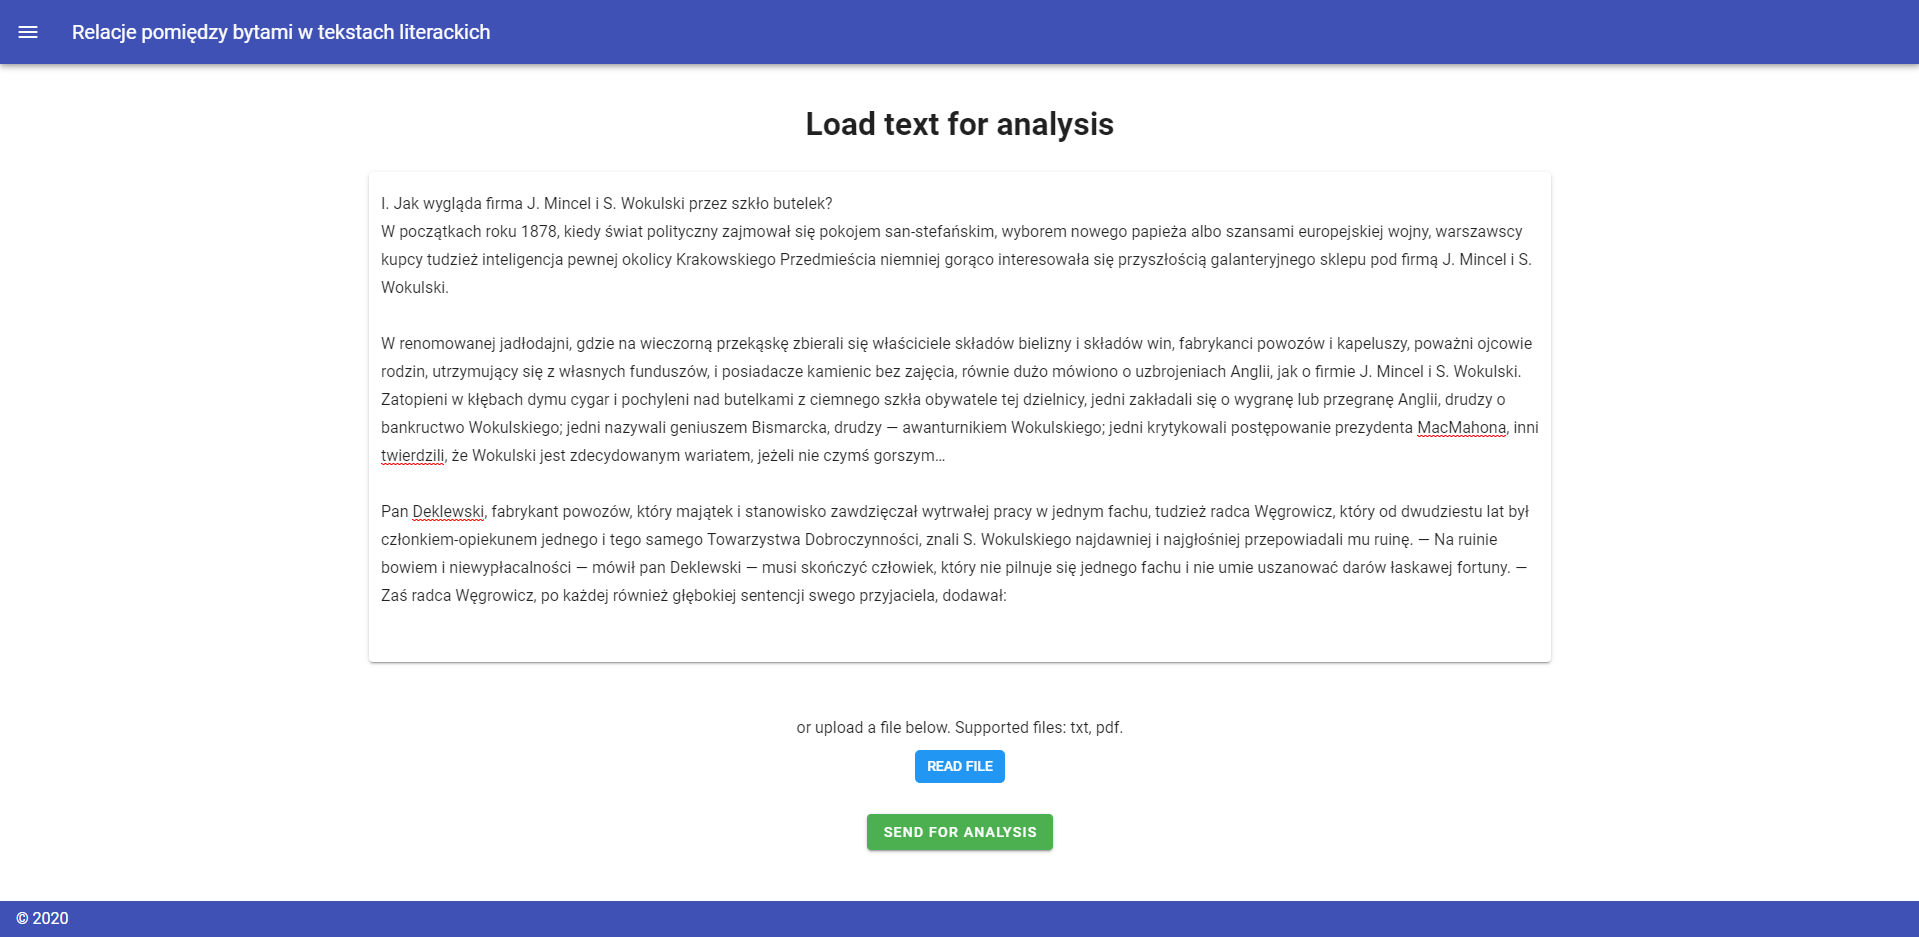
\includegraphics[width=0.9\textwidth]{rys/upload-tekstu.png}}
                \caption{Interfejs wczytywania tekstu}
            \end{figure}
            
        \subsubsection{Dane}
            Cały tekst książki pakowany jest w JSONa i wysyłany metodą \texttt{POST} na endpoint wystawiony przez backend. Ten endpoint zwraca wtedy \texttt{ID} dokumentu w bazie danych. Ten \texttt{ID} używany jest przez podstronę wyświetlająca dane. Zaraz po wysłaniu backend rozpoczyna analizę tekstu oznaczając to stosownym statusem w bazie danych. Gdy analiza jest zakończona status ulega zmianie i możliwe jest pobranie danych grafu przez podstronę służącą do wizualizacji.
            
            Pobranie tych danych polega na wysłaniu zapytania typu \texttt{GET} na ten sam endpoint. Gdy dane nie są gotowe, zwracany jest tylko odpowiedni status, a podstrona informuje stosownym komunikatem. Gdy analiza jest zakończona zwracane są dane grafu, które zostają wyświetlone.
            
    \subsection{Prezentacja danych}

        \subsubsection{Metoda prezentacji danych}
            Do prezentacji wygenerowanych relacji został wybrany graf skierowany siłą (ang. \textit{force-directed graph}).
            Algorytm rysowania takiego grafu wykorzystuje jedynie informacje zawarte w strukturze danych (węzły oraz połączenia między nimi).
            Grafy wygenerowane za pomocą takich algorytmów są estetyczne i uporządkowane. Posiadają także niewielką ilość przecinających się połączeń \cite{yeet}. Te cechy są szczególnie przydatne w przypadku wizualizowania dużych zbiorów danych. Generowanie grafu polega na przypisaniu sił między zbiorem krawędzi i zbiorem węzłów w oparciu o ich względne pozycje, a następnie użyciu tych sił do symulacji ruchu krawędzi i węzłów lub do zminimalizowania ich energii\cite{yworks}. W pierwszym przypadku siły są liczone w czasie rzeczywistym, czego wynikiem jest graf, w którego układ może ingerować użytkownik (np. poprzez przeciąganie węzłów w inne pozycje). W drugim przypadku wyświetlenie grafu następuje po zminimalizowaniu sił, czego wynikiem jest statyczny graf. Odświeżanie widoku grafu w czasie rzeczywistym znacząco zwiększa czas minimalizacji sił, ponieważ widok grafu jest często odświeżany. Graf statyczny osiąga minimalne siły w dużo krótszym czasie, jednak pozbawiony jest możliwości interakcji z węzłami. W projekcie została zaimplementowana pierwsza metoda, ponieważ kluczowa jest ingerencja użytkownika w pozycje wierzchołków grafu.\\
            
            Do generowania grafu została wykorzystana biblioteka D3.js \cite{d3}. Wybór biblioteki jest umotywowany wysoko konfigurowalną implementacją grafu skierowanego siłą.
    
            \begin{figure}[h]
            \caption{Wygenerowany graf współwystępowania postaci w Les Mis\'erables}
            \frame{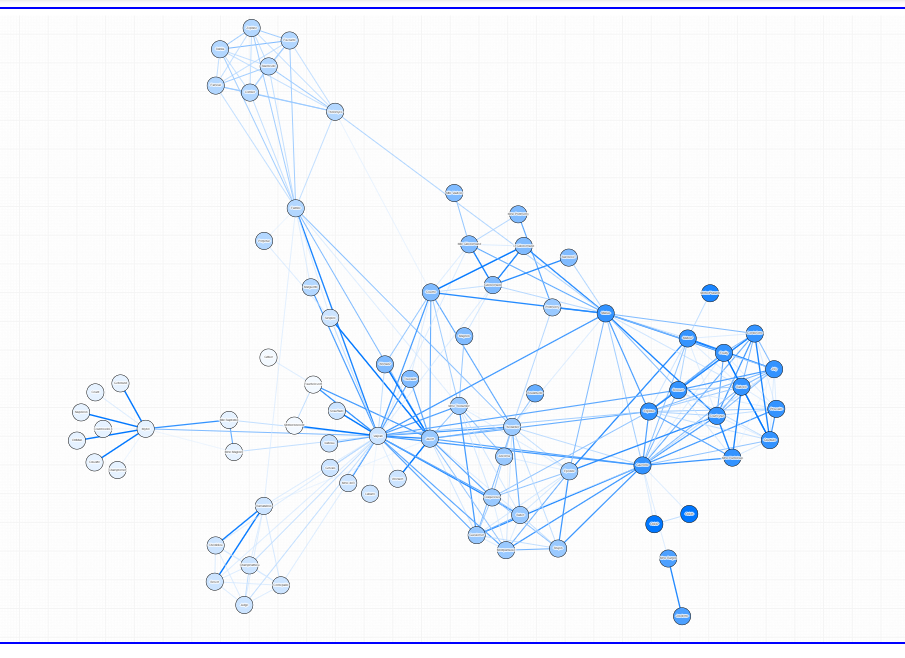
\includegraphics[width=13cm]{rys/graph.png}}
            \label{fig:graph}
            \centering
            \end{figure}
            
        \newpage
        \subsubsection{Metoda prezentacji relacji bytów}

            Relacje bytów zostały zobrazowane poprzez zmienny kolor oraz grubość połączenia między poszczególnymi bytami. Im mocniejsza relacja między bytami, tym połączenie jest grubsze oraz posiada bardziej intensywny kolor [rys~\ref{fig:links}].
            
            \begin{figure}[h]
            \caption{Wizualizacja relacji bytów}
            \frame{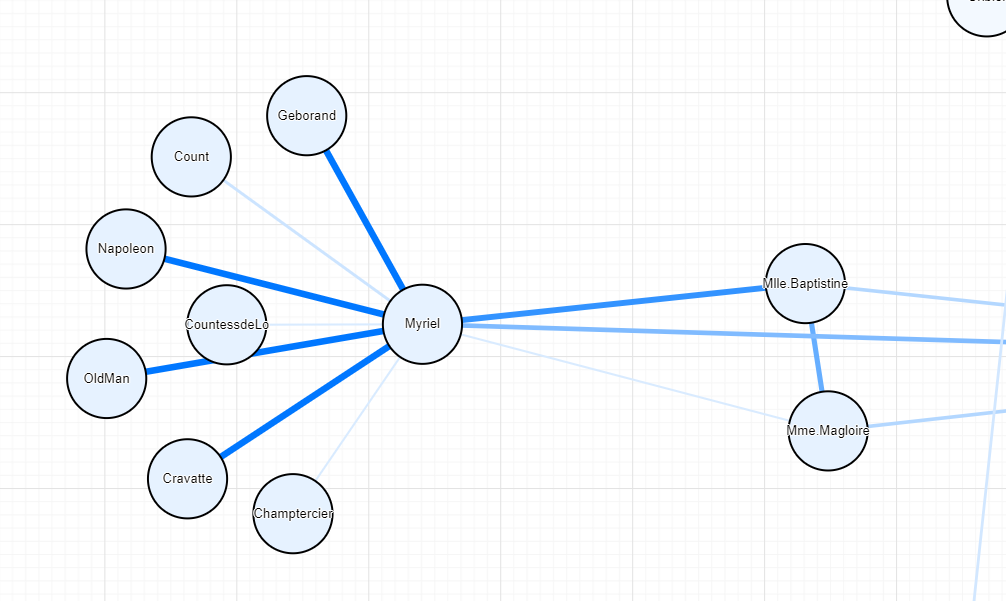
\includegraphics[width=13cm]{rys/links.png}}
            \label{fig:links}
            \centering
            \end{figure}
            
            Dodatkowo, wierzchołki reprezentujące byty posiadają kolor zależny od częstości ich występowania. Im częściej dany byt pojawia się w analizowanym teście, tym bardziej intensywny kolor wierzchołka [rys~\ref{fig:nodes}].
            
            \begin{figure}[h]
            \caption{Wizualizacja częstości występowania bytów}
            \frame{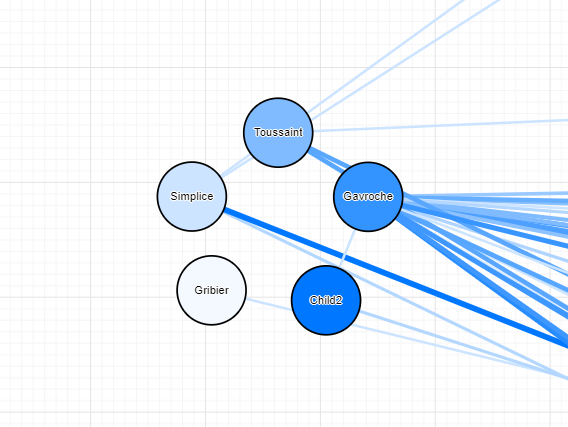
\includegraphics[width=12cm]{rys/nodes.png}}
            \label{fig:nodes}
            \centering
            \end{figure}
            
    \subsection{Dostępne akcje w reprezentacji graficznej}
        \subsubsection{Akcje w obrębie pola grafu}
            W celu zapewnienia większej czytelności zostały zaimplementowane następujące funkcjonalności:
            \begin{itemize}
                \item przybliżanie oraz oddalanie widoku kółkiem myszy,
                \item przesuwanie widoku poprzez przeciąganie tła myszą.
                \item zaznaczanie połączonych węzłów po najechaniu myszą [rys~\ref{fig:highlight}]
                \item przeciąganie węzłów
            \end{itemize}
            
            \begin{figure}[h]
            \caption{Zaznaczenie pojedynczego bytu}
            \frame{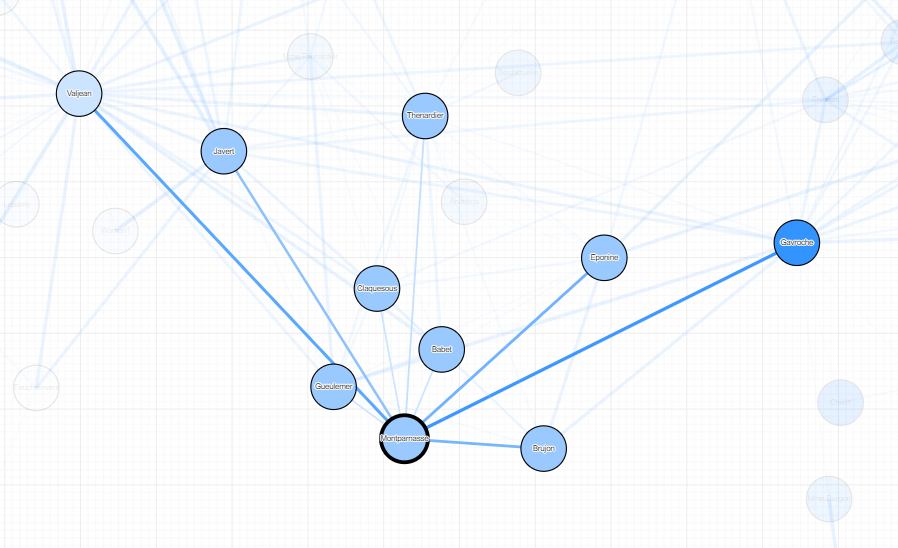
\includegraphics[width=9cm]{rys/highlight.png}}
            \label{fig:highlight}
            \centering
            \end{figure}
        
        \subsubsection{Modyfikowanie parametrów wyświetlania grafu}
        
            Użytkownik ma możliwość zmiany następujących parametrów wyświetlanego grafu:
            \begin{itemize}
                \item Włączanie i wyłączanie sił w grafie -- Podczas gdy siły są wyłączone, użytkownik może dowolnie przestawiać wierzchołki[rys~\ref{fig:forceOff}].
                \item Zmiana sprężystości grafu -- Modyfikacja tego parametru zmienia siłę oddziałującą na wierzchołki grafu.
                \item Czułość krawędzi -- możliwość określenia jak bardzo znaczące krawędzie będą wyświetlane
                \item Czułość wierzchołków -- możliwość określenia jak bardzo znaczące wierzchołki będą wyświetlane
            \end{itemize}
            
            \begin{figure}[h!]
            \centering
            \begin{subfigure}{.45\textwidth}
              \centering
              \fbox{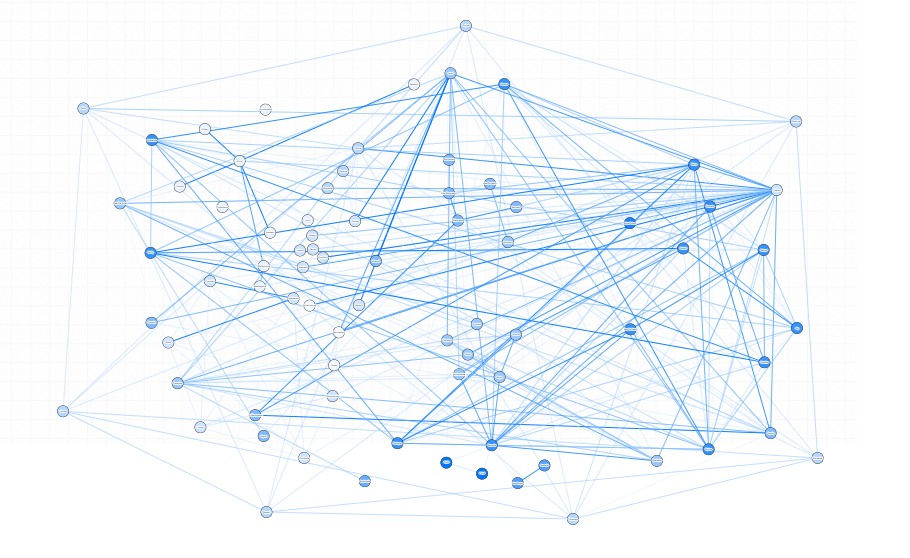
\includegraphics[width=.9\linewidth]{rys/forceOff.png}}
            \end{subfigure}
            \begin{subfigure}{.45\textwidth}
              \centering
              \fbox{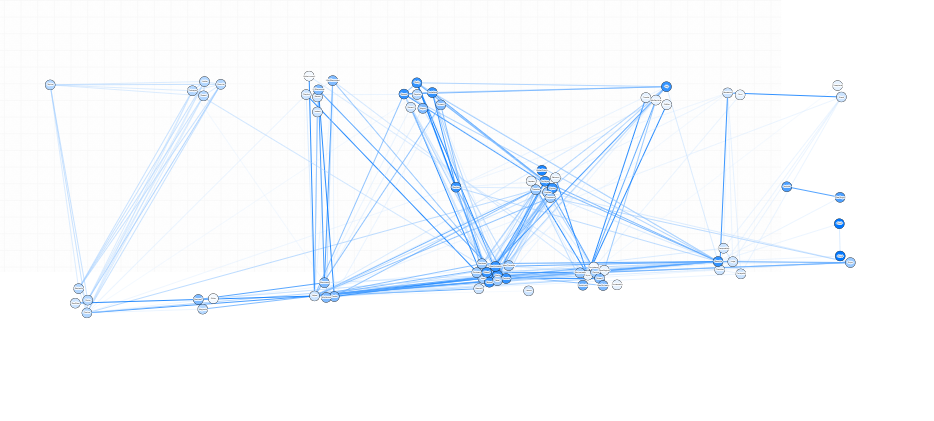
\includegraphics[width=.9\linewidth]{rys/forceOff2.png}}
            \end{subfigure}
            \caption{Przestawione wierzchołki po wyłączeniu sił}
            \label{fig:forceOff}
            \end{figure}
            
        \subsubsection{Łączenie mylnie rozdzielonych bytów}
            
            Użytkownik posiada możliwość ręcznego złączenia dwóch bytów w jeden [rys~\ref{fig:input}]. Funkcjonalność ta jest przydatna w przypadku gdy narzędzie analizujące tekst mylnie rozróżni jeden byt jako dwa osobne. Łączenie bytów polega na usunięciu pierwszego z nich oraz przypisaniu odpowiednich połączeń do bytu drugiego. Wynik takiej operacji został przedstawiony na rysunku \ref{fig:merge}. Wszelkie zmiany dokonane przez użytkownika mogą zostać przywrócone przyciskiem \textit{Przywróć zmiany}. W celu zwiększenia przejrzystości, byt który ma zostać włączony do drugiego zmienia kolor na czerwony oraz byt który ma zostać pozostawiony zmienia kolor na zielony.
    
            \begin{figure}[h!]
            \centering
            \begin{subfigure}{.45\textwidth}
              \centering
              \fbox{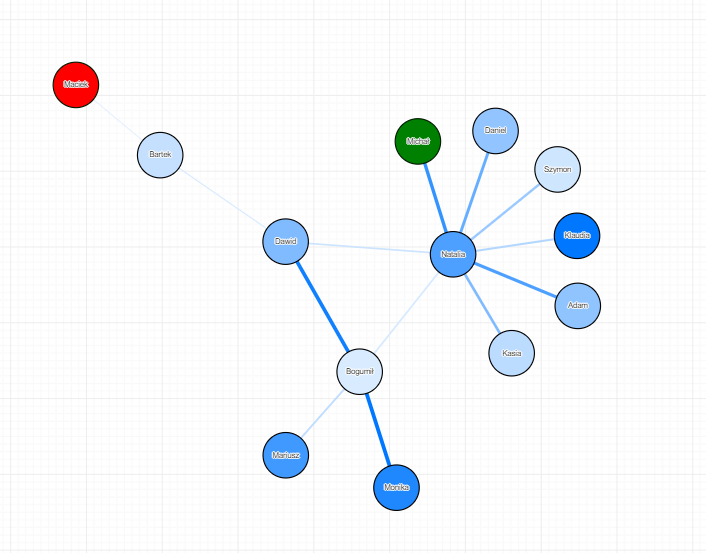
\includegraphics[width=.9\linewidth]{rys/merge_before.png}}
              \caption{Przed złączeniem}
            \end{subfigure}
            \begin{subfigure}{.45\textwidth}
              \centering
              \fbox{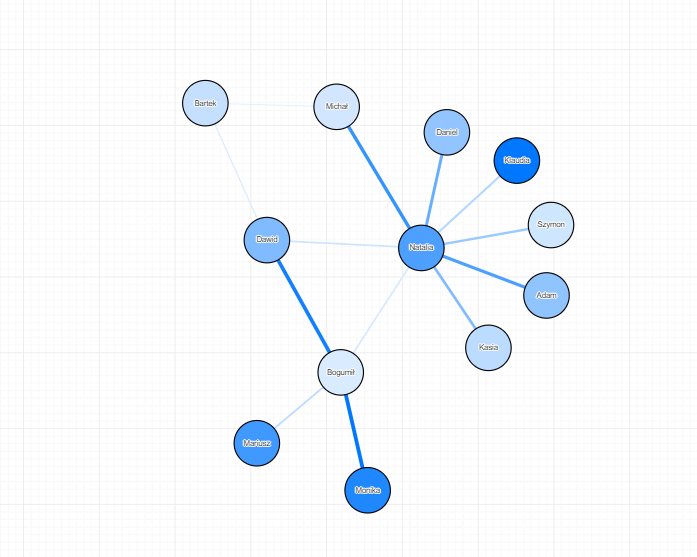
\includegraphics[width=.9\linewidth]{rys/merge_after.png}}
              \caption{Po złączeniu}
            \end{subfigure}
            \caption{Efekt złączenia bytów}
            \label{fig:merge}
            \end{figure}
        
            
            \begin{figure}[h!]
            \centering
            \begin{subfigure}{.45\textwidth}
              \centering
              \fbox{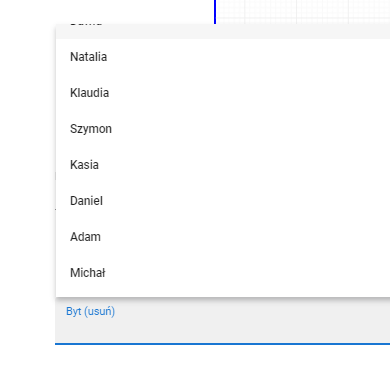
\includegraphics[width=.9\linewidth]{rys/nodes_list.png}}
              \caption{Lista}
            \end{subfigure}
            \begin{subfigure}{.45\textwidth}
              \centering
              \fbox{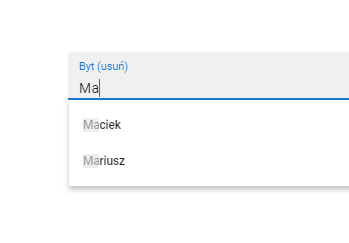
\includegraphics[width=.9\linewidth]{rys/nodes_autocompletion.png}}
              \caption{Autouzupełnianie}
            \end{subfigure}
            \caption{Wybór bytów do złączenia}
            \label{fig:input}
            \end{figure}
            
        \subsection{D3.js - biblioteka wizualizacji danych}
        
            D3.js to znacznie więcej niż biblioteka do wizualizacji, a raczej całe podejście do tworzenia dokumentów opartych na danych. Nie jest to monolit, D3 w obecnej wersji jest biblioteką modułową, zawiera w sobie szereg narzędzi wspomagających operacje na danych: takich jak przygotowanie skali, renderowanie wykresów, grafów i map. Biblioteka ta pozwala na dodanie animacji, stylów i customowych zachowań.
            D3.js jest bardzo uniwersalne ale przychodzi to kosztem dużej inwestycji w naukę biblioteki i zrozumienia powiązań wszystkich modułów. Dzięki podejściu D3.js cała biblioteka jest niezwykle lekka, biorąc pod uwagę możliwości. W najnowszej wersji waży niewiele ponad 70kB w wersji min. Wiele innych bibliotek bazuje na D3.js, rozszerzając pewne funkcje, często specjalizując się i ułatwiając konkretne aspekty wizualizacji danych. 
            
        \subsection{Zapis do plików}
            Do zapisania aktualnego stanu modelu do pliku wykorzystane zostało API przeglądarki do wygenerowania pliku, który następnie jest pobierany. 
            
            \subsubsection{Zapis modelu wykresu do pliku GDF}
                GDF to format tekstowy przypominający CSV. Pozwala definiować węzły oraz krawędzi grafu. Wspiera przechowywanie wielu atrybutów o różnych typach i odnoszących się zarówno do krawędzi, jak i węzłów. Opis grafu w tym formacie może zostać zaimportowany do narzędzia \emph{Gephi}.\\
                Plik składa się z dwóch sekcji:
                \begin{itemize}
                    \item definicje węzłów,
                    \item definicje krawędzi
                \end{itemize}
                Każda z sekcji posiada swój nagłówki w formacie:
                \begin{itemize}
                \item \lstinline{nodedef> atr1 typ1, atr2 typ2, ...}
                \item \lstinline{edgedef> atr1 typ1, atr2 typ2, ...}
                \end{itemize}
                w naszym przypadku jest to:
                \begin{itemize}
                \item \lstinline{nodedef> name VARCHAR, label VARCHAR, class VARCHAR, value DOUBLE}
                \item \lstinline{edgedef> source VARCHAR, target VARCHAR, type VARCHAR, value DOUBLE}
                \end{itemize}
                Poniżej nagłówków znajdują się deklaracje poszczególnych krawędzi oraz węzłów składające się z atrybutów zdefiniowanych w nagłówku rozdzielonych przecinkami. Każdy wiersz odpowiada jednemu elementowi grafu.
                
            \subsubsection{Zapis modelu wykresu do pliku JSON}\label{json}
                %tutej WOJTEG
                \paragraph{Format}\\
                
                Dane zwracane przez funkcje parsująca zawierają się w formacie danych JSON. Format prezentuje się następująco:
        \begin{lstlisting}
{
   "nodes": [
      {
         "name": "Pawel",
         "occurrence": 50
      },
      {
         "name": "Przemek",
         "occurrence": 45
      },
      {
         "name": "Wojtek",
         "occurrence": 25
      },
      ...
   ],
   "links": [
      {
         "source": 0,
         "target": 1,
         "value": 67,
      },
      {
         "source": 0,
         "target": 2,
         "value": 15,
      },
      {
         "source": 0,
         "target": 3,
         "value": 98,
      },
      ...
   ]
}
        \end{lstlisting}
        
        Sekcja \textit{nodes} odpowiada za przekazanie danych wszystkich węzłów bytów wraz z ich nazwami(name) oraz sklasyfikowaną po stronie backendu częstością występowania(occurrence). Częstość występowania zależna jest od maksymalnej wartości występowania postaci.\\
        
        Sekcja \textit{links} odpowiada za informacje dotyczące własności połączeń. Opisuje ona między którymi wierzchołkami następuje połączenie(source i target), wartość value, która określa moc połączenia(im większa tym silniejsze połączenie). Moc połączeń jest klasyfikowana odnosząc się do maksymalnej wartości połączenia.
            
            \subsubsection{Eksport wykresu do pliku graficznego}
            
                Eksport wykresu odbywa się poprzez generowanie pliku PNG przez przeglądarkę. Jest on generowany na podstawie obecnej zawartości tagu \textit{<svg>} w którym znajduje się renderowany wykres. Plik graficzny zawiera legendę oraz wszystko co jest widoczne na wykresie w czasie kliknięcia przycisku \textit{Zapisz graf do pliku graficznego}. Takie działanie umożliwia ustawienie grafu w odpowiadającym użytkownikowi stanie i eksport tego grafu, jego części lub zbliżenia na daną część do pliku graficznego.
            %to chyba też było już gdzieś opisane

            
        \subsection{Odczyt z pliku}
            %tutaj update plus metoda Pawła
                            
                Struktura pliku jest identyczna do tej opisanej w rozdziale \ref{json}. Przy wczytywaniu z pliku użytkownik wybiera plik z dysku z danymi wykresu.
                \begin{figure}[!h]
                    \center
                        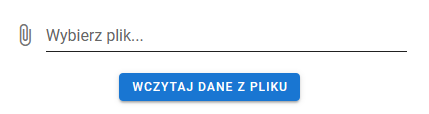
\includegraphics[scale=1]{rys/wojtek/1.png}
                        \caption{Element UI odpowiadający za wczytanie danych grafu}
                        \label{UIloadFile}
                \end{figure}
                W przypadku gdy ktoś niepoprawnie wypełni pole z wyborem pliku i kliknie przycisk {Wczytaj dane z pliku} zostanie mu wyświetlona informacja ukazana na rysunku \ref{uidialog}
                
                \begin{figure}[!h]
                    \center
                        
\includegraphics[scale=1]{rys/wojtek/2.png}
                        \caption{Komunikat informujący o braku pliku do wczytania}
                        \label{uidialog}
                \end{figure}
        
        \subsection{Lista grafów}
            %opis jakie grafy są
        Po wczytaniu tekstu zostaje on zapisany w bazie danych na serwerze. W zakładce znajduje się lista z wygenerowanymi już grafami. Można je przeglądać i otwierać. Po wybraniu i kliknięciu w interesujący nas graf, zostajemy przeniesieni do jego wizualizacji. Tam możemy dokonać jego przekształceń, edycji oraz zapisu do pliku.
        
        
        \begin{figure}[h!]
                \centering
                \fbox{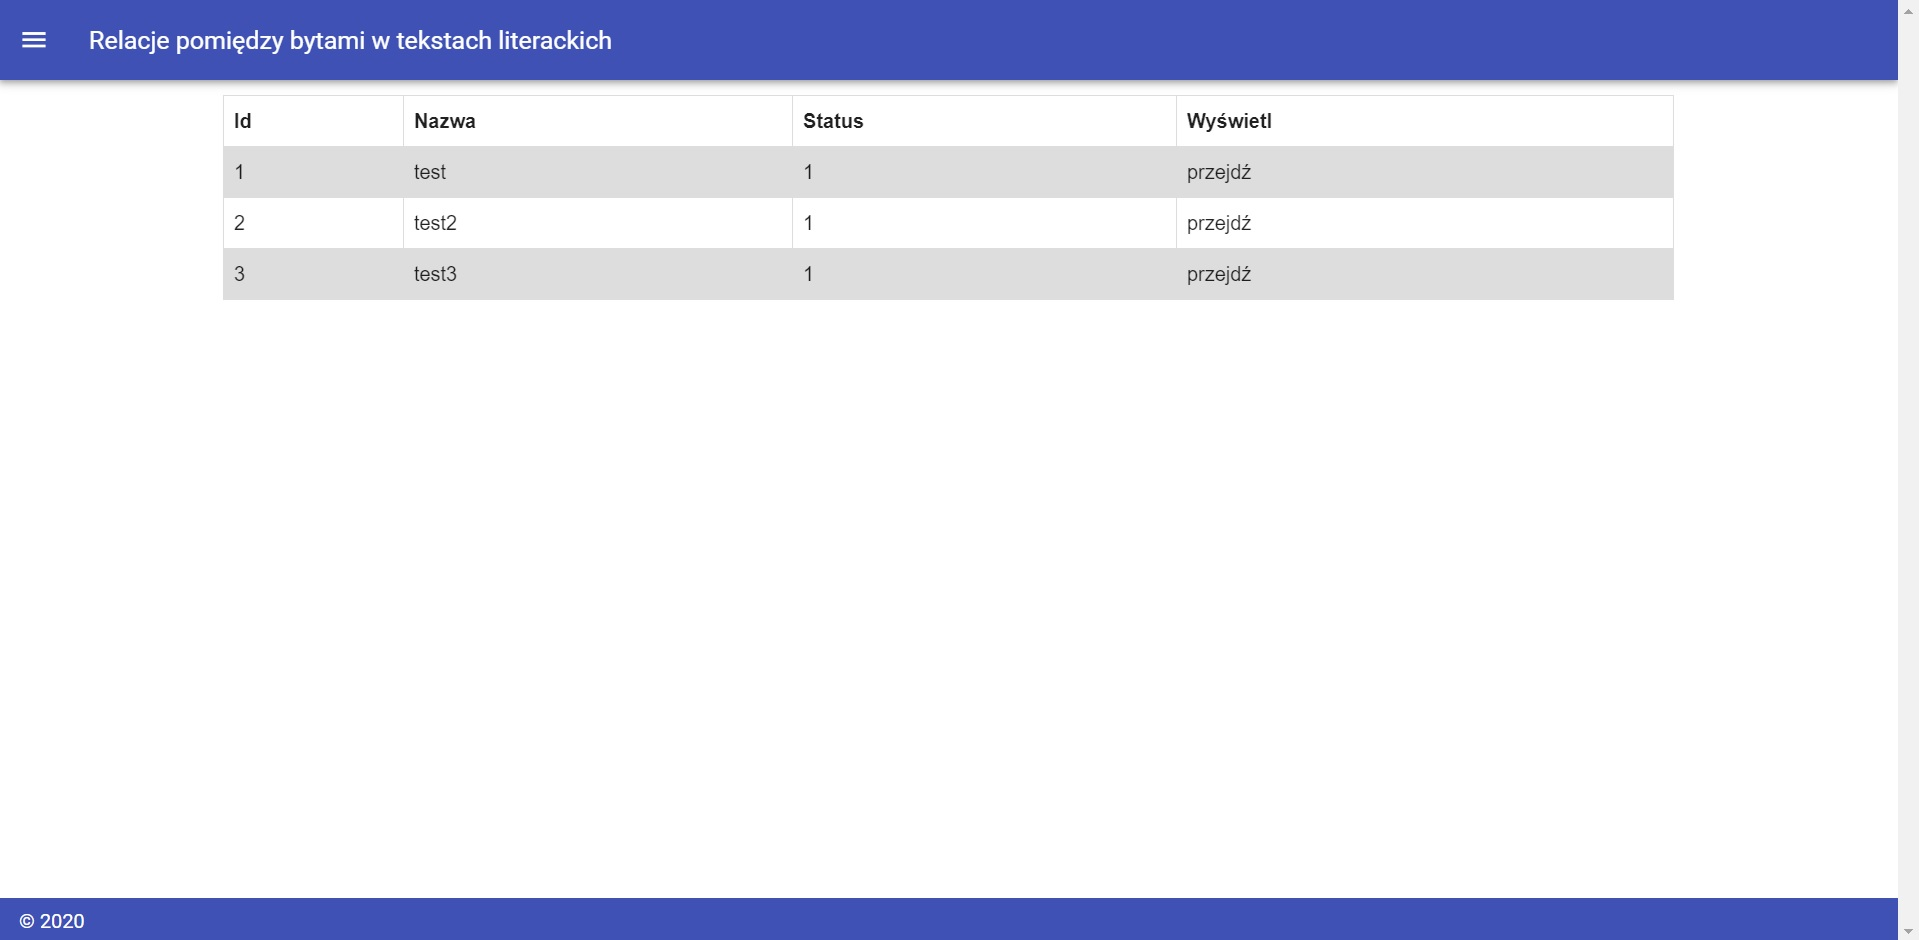
\includegraphics[width=0.9\textwidth]{rys/graphlist.jpg}}
                \caption{lista wygenerowanych grafów}
            \end{figure}
   

\newpage
    \subsection{Metoda szukania powiązania}
        % coś o doborze wagno, tutaj obrazki są 
        % https://docs.google.com/spreadsheets/d/1PjEAjZ1F2Kp4x7HSWIRXJG0aGkV7MQFsJRegS8vWMEA/edit#gid=0
        Ekstrakcja bytów z przeanalizowanego tekstu odbywa się z wykorzystaniem narzędzia \textit{NER}. W wynikowym pliku XML zliczane są wystąpienia wszystkich tagów oznaczonych kategoriami:
        \begin{itemize}
            \item subst -- rzeczownik,
            \item m1 -- męskoosobowy,
            \item m2 -- męskożywotny,
            \item f -- żeński,
            \item n -- nijaki,
        \end{itemize}
        oraz zawierające pole \emph{nam\_liv} z wartością większą od 0.\\
        
        Opracowano dwa warianty algorytmu polegającego na wydzielaniu z XML-a bytów występujących w poruszającym się po tekście oknie o zmiennej wielkości.
        
        W pierwszej metodzie algorytm rozpoczyna się od zsumowania wystąpień wszystkich bytów w całym wprowadzonym tekście, następnie dokonuje się podziału tekstu na pół. W otrzymanych częściach liczone są wystąpienia bytów. Czynność jest powtarzana aż do osiągnięcia fragmentów tekstu wielkości jednego zdania. Schemat podziału tekstu pokazano na rysunku \ref{fig:polowy}. Wystąpieniom bytów w danym etapie analizy (rozmiar analizowanego fragmentu tekstu) przydzielane są wagi według określonej charakterystyki (stała, liniowa, kwadratowa, etc.) zachowując prawidłowość: im mniejszy analizowany fragment tekstu, tym większa waga.
        \begin{figure}[!h]
        \caption{Metoda Pierwsza, podział tekstu}
        \frame{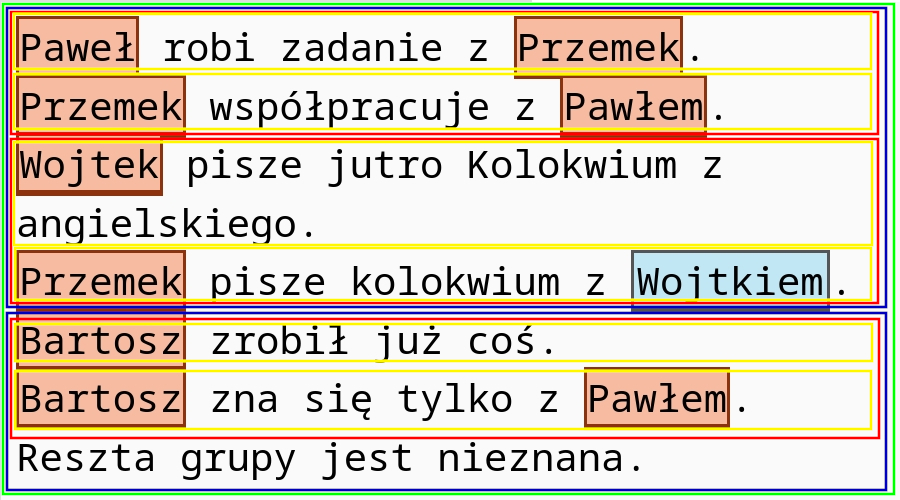
\includegraphics[width=14cm]{rys/polowy.jpg}}
        \label{fig:polowy}
        \centering
        \end{figure}
        
        Druga metoda polega na przemieszczaniu okna po tekście począwszy od pierwszego zdania, aż do końca tekstu w krokach co jedno zdanie, tak jak zaprezentowano na rysunku \ref{fig:plyw}. W każdym kroku, z tekstu znajdującego się w obrębie okna, wydzielane i sumowane będą wystąpienia poszczególnych bohaterów utworu. Każdemu wystąpieniu przydzielana jest waga zależna od rozmiaru okna -- po zakończeniu analizy oknem o największym rozmiarze następuje zmniejszenie okna oraz zwiększenie wagi wystąpienia bytu i powtórzenie analizy z nowym oknem -- większą wagę będą miały dwa byty występujące na obszarze dwóch zdań, niż inne, przeanalizowane na etapie okna o rozmiarze np. 50 zdań. Wystąpienia postaci w obrębie jednego rozmiaru okna, wraz z ilością wystąpień, charakteryzują relację między tymi postaciami. Po osiągnięciu rozmiaru okna równego jednemu zdaniu, relacje pomiędzy bytami z wszystkich etapów są sumowane z uwzględnieniem wag, co daje finalny efekt.
        \begin{figure}[!th]
        \caption{Metoda Druga, podział tekstu}
        \frame{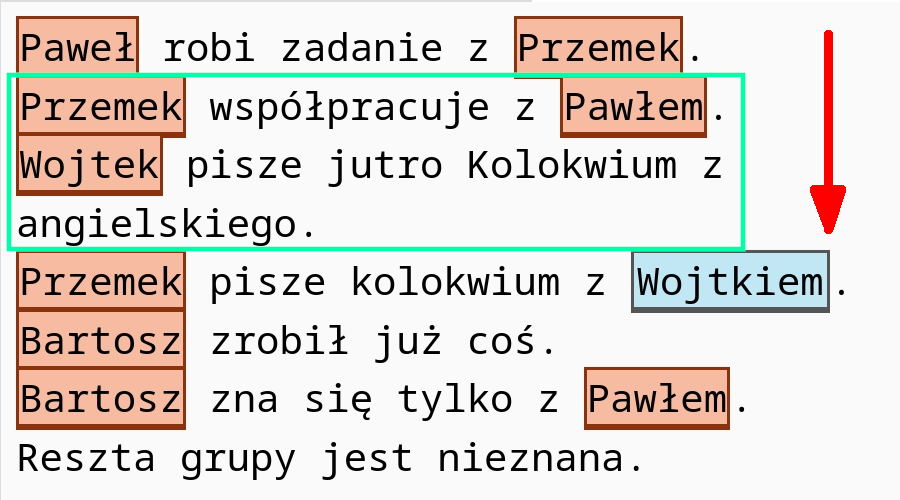
\includegraphics[width=14cm]{rys/plyw.jpg}}
        \label{fig:plyw}
        \centering
        \end{figure}
        
         Raz wygenerowane z narzędzia \textit{NER} pliki XML zostają poddane analizie przez algorytm, a wyniki są zapisywane w formacie JSON i przechowywane w serwerze.
        
        
        %\newpage
        %\printbibliography

\end{document}

%xDDDDDD